\documentclass{report}
\usepackage[utf8]{inputenc}
\usepackage{svg}
\usepackage{float}
\usepackage{graphicx}
\usepackage{verbatim}
\usepackage{geometry}
\geometry{a4paper, margin=1in}

\title{Descriptif des développements logiciels}
\date{25/03/2025}

\begin{document}

\maketitle

\section*{\centering Contexte et objectifs}
\vspace{0.5cm}
\noindent EcoDeli est une entreprise de mise en relation entre clients et prestataires de services. Son objectif principal est d’optimiser la logistique des livraisons tout en réduisant les coûts et l’empreinte carbone, en utilisant les trajets des particuliers et/ou professionnels déjà prévus. Avec le temps, elle a également élargi son offre en proposant un réseau de prestataires pour divers services (transport, installations, entretien, etc.). \\

\noindent Ce document détaille le descriptif technique du projet en termes de développement informatique sur les différentes applications commandées par l’entreprise :
\begin{itemize}
    \item \textbf{Application web (public)}
    \item \textbf{Application mobile (public)}
    \item \textbf{Application back-office (interne)}
    \item \textbf{Application info-centre (interne)}
\end{itemize}
\vspace{0.4cm}
\noindent Les application doivent offrir une interface utilisateur ergonomique et sécurisée permettant d’assurer l’intermédiation pour les prestations de service et l'administration. Elle se doivent d'être développées de manière évolutives et durables pour accompagner la croissance de l’entreprise. 
\vspace{1cm}

\section*{\centering Spécifications fonctionnelles}
\vspace{0.5cm}
\subsection*{1. Authentification}
\vspace{0.2cm}
\noindent L’analyse des besoins a permis d’identifier et de segmenter les utilisateurs en profils distincts. La première différentiation fut de les divisés en deux grandes catégories : \textbf{clients et collaborateurs}. Un client utilise l’application web et mobile avec des fonctionnalités adaptées à son profil tandis qu'un collaborateur quant à lui, a accès au back-office (via une interface web) ou à l’application de visualisation de données. \\

\noindent En ce qui concerne les collaborateurs, ils disposent du statut d'\textbf{administreur} à qui l'accès à l'application web en tant que client est impossible. Pour accéder au back-office, un compte doit avoir été créé au préalable car il n'existe pas auto-inscription de même pour l'application de visualisation de données, installée directement en client lourd sur les machines des employés. \\

\noindent Pour un client, l'accès à l'application commence par une connexion à un compte existant ou une inscription afin de se créer un compte. Lors de l'inscription, l'utilisateur est catégorisé en fonction de son statut, \textbf{particulier ou professionnel}. Cette première différenciation est irrémédiable et entraîne une vérification dans le cas où l'utilisateur choisit le statut professionnel. \\

\noindent Un second choix, non irréversible, s'offre à l'utilisateur : il peut décider s'il souhaite uniquement être un \textbf{client de services} ou s'il souhaite également pratiquer la \textbf{prestation de services}. Dans ce dernier cas, toute prestation de service nécessite aussi une vérification. Lors de l'inscription, l'utilisateur choisit qu'une prestation mais il pourra en ajouter d'autres par la suite, sauf particulier ou la seule prestation accessible est la livraison de colis. \\

\noindent Ensuite l'inscription se poursuit avec une série d'informations à fournir pour finaliser le processus en fonction des choix précédents. Par exemple, des informations personnelles pour un particulier ou des informations relatives à l'entreprise pour un professionnel, ou selon la prestation choisie à l'inscription, des documents supplémentaires pour attester des qualifications de l'utilisateur. Après inscription, le compte de l'utilisateur est donc initialement bloqué et nécessite une validation par un administrateur sauf pour particulier non-prestataire. \\

\noindent À la première connexion un overlay bloquant est affiché pour expliquer aux nouveaux clients les différents onglets et actions disponibles. Aussi en cas d'oubli de son mot de passe, l'utilisateur peut proceder à une demande de réinitialisation via son adresse email. \\

\noindent On termine donc avec cinq profils différents d'utilisateurs :
\begin{itemize}
    \item \textbf{L’administrateur :} Collaborateur
    \item \textbf{Le client particulier :} Client $\rightarrow$ Particulier $\rightarrow$ Client de services
    \item \textbf{Le client professionnel :} Client $\rightarrow$ Professionnel $\rightarrow$ Client de services
    \item \textbf{Le prestataire particulier :} Client $\rightarrow$ Particulier $\rightarrow$ Prestataire de services
    \item \textbf{Le prestataire professionnel :} Client $\rightarrow$ Professionnel $\rightarrow$ Prestataire de services
\end{itemize}
\vspace{0.5cm}

\subsection*{2. Prestations} 
\vspace{0.2cm} 
\noindent Le cœur de métier d’Ecodeli repose sur l’intermédiation dans la prestation de services, répondant aux besoins des particuliers et des professionnels. Nous avons structuré cette offre en deux axes principaux : \\

\noindent \textbf{Les livraisons solidaires :} Service de transport écologique visant à optimiser l’empreinte carbone en exploitant les trajets déjà prévus par des particuliers ou des professionnels. Un utilisateur souhaitant expédier un colis peut publier une annonce en précisant l’adresse de départ et de destination. Les livreurs habilités peuvent alors consulter ces annonces et se positionner pour effectuer la livraison. \\

\noindent Par ailleurs, les livreurs ont également la possibilité d’indiquer à l’avance leurs trajets et lorsqu’une annonce est déposée, un traitement automatique analyse les trajets disponibles et propose la livraison aux livreurs correspondants. Si une livraison nécessite plusieurs segments, le colis peut être temporairement stocké dans un entrepôt d'Ecodeli avant d’être acheminé par un autre livreur. Le client est ensuite débité lors de l’acceptation de sa demande par un livreur, puis remboursé en cas de désistement, quant au livreur, il est rémunéré à la fin de la livraison, sous réserve de l’absence de litige. 
\vspace{0.2cm}
\begin{figure}[H]
    \centering
    \includesvg[height=9cm]{delivery.svg}
    \caption{cycle de vie d'une annonce pour livraison}
\end{figure}
\vspace{0.5cm}
\noindent \textbf{Les prestations de services :} Ce volet est plus complexe, car il repose sur un processus d’habilitation et d’évolution des offres de services. Bien que la livraison soit un service à part entière, elle a été distinguée des autres prestations en raison du statut spécifique des livreurs, qui peuvent être aussi bien des particuliers que des professionnels.
\begin{itemize}
    \item Un administrateur crée initialement chaque service, avec la possibilité pour les utilisateurs de proposer des évolutions.
    \item Chaque service nécessite une habilitation, obtenue en fournissant des documents justificatifs exigés lors de la création du service.
    \item Une fois habilité, le prestataire publie des annonces en indiquant ses créneaux de disponibilité ainsi que son tarif horaire.
    \item Les clients peuvent ensuite faire une demande sur ces annonces et se positionner pour la prestation.
    \item Le prestataire a la possibilité d’accepter la demande ou de proposer des ajustements.
    \item Dès qu’une demande est faite, un canal de communication est automatiquement créé entre le client et le prestataire pour faciliter la négociation.
\end{itemize}
\vspace{1cm}

\section*{\centering Spécifications techniques}
\vspace{0.5cm}
\subsection*{1. Vue d’ensemble}
\vspace{0.2cm}
\noindent Pour mener à bien les développements des différents produits, le stack technique mis en place comprend plusieurs technologies adaptées à chaque partie. \\

\noindent Le front-end web est développé avec Next.js et React.js, en utilisant Tailwind CSS pour la gestion des styles. Pour le front-end mobile, l'application utilise Kotlin pour la partie native, avec OneSignal pour les notifications. En ce qui concerne le front-end data, la technologie n'a pas encore été définie. \\

\noindent Le back-end est construit à l'aide de Java et Spring Boot, un choix qui permet de bénéficier de la robustesse et de la flexibilité de ce framework. Pour la gestion des données, nous avons opté pour PostgreSQL comme base de données SQL et MongoDB pour la gestion des données NoSQL. \\

\noindent Concernant l'authentification et la sécurité, l'accès aux applications est géré via JWT (JSON Web Tokens) pour une gestion fine des droits d'accès, avec un stockage sécurisé des clés et informations sensibles via Azure Key Vault. Conteneurisée à l'aide de Docker, une pipeline CI/CD est aussi mise en place avec Azure DevOps, facilitant l'intégration continue et le déploiement automatisé. Enfin, l'hébergement choisi pour l'environnement de test est Azure Cloud tandis qu'en production les applications seront hébergés sur l'infrastructure dédié d'EcoDeli. \\
\vspace{0.5cm}

\subsection*{2. Modèle de données}
\vspace{0.2cm}
\noindent Hormis la gestion des messages et des traductions , toutes les applications reposent sur une base de données relationnelle, structurée de manière à répondre aux exigences fonctionnelles. La méthode employée pour la conception de la base repose sur une approche relationnelle et modulaire, garantissant ainsi une scalabilité, une évolutivité et une maintenabilité optimisées. L’objectif principal est de permettre l’ajout de nouveaux services et fonctionnalités sans perturber l’architecture existante. \\

\noindent Le choix d’un double système de gestion de bases de données repose sur des besoins fonctionnels distincts. \textbf{PostgreSQL} est utilisé pour gérer l’ensemble des entités relationnelles, offrant une gestion robuste et cohérente des données structurées. En parallèle, \textbf{MongoDB} est utilisé pour le stockage rapide et flexible des messages échangés en temps réel et des traductions, en raison de leur nature non structurée et de leur volume élevé. Cette combinaison garantit une efficacité optimale dans la gestion des données tout en respectant les contraintes de performance et de flexibilité.
\vspace{0.2cm}
\begin{figure}[H]
    \centering
    \includesvg[height=7.5cm]{mcd.svg}
    \caption{modèle conceptuel des données}
\end{figure}
\begin{figure}[H]
    \centering
    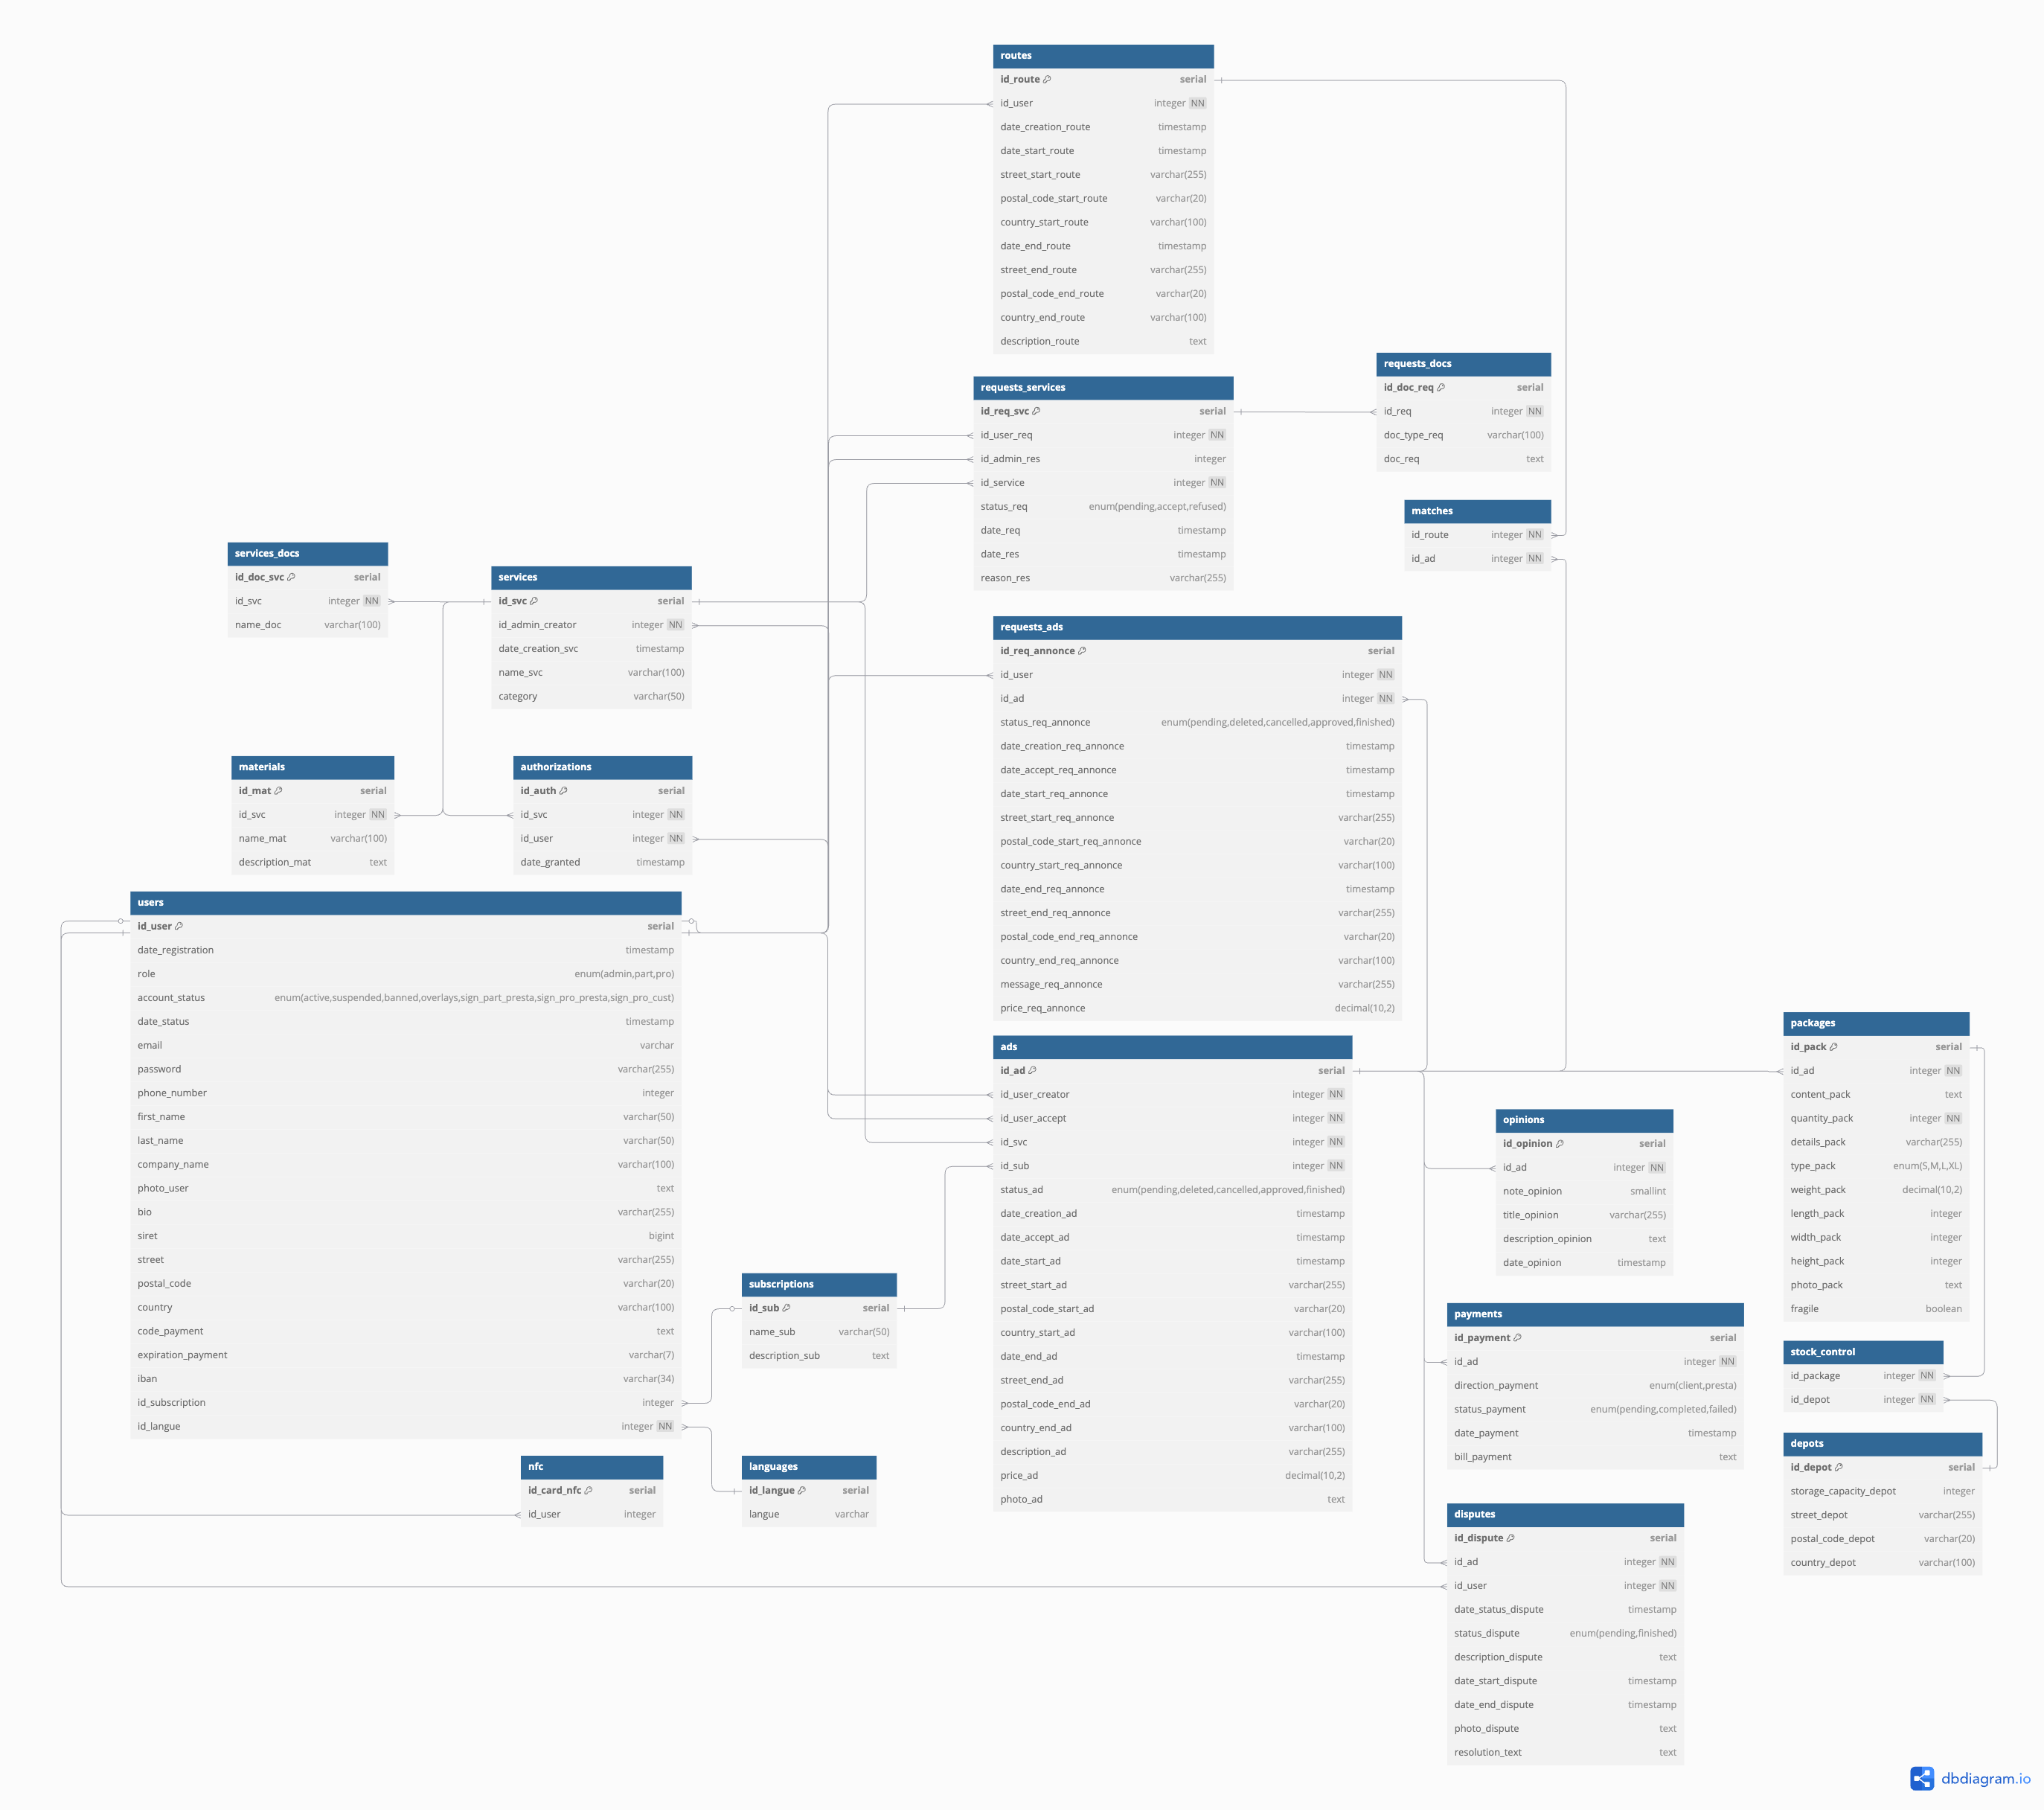
\includegraphics[height=12cm]{mld.png}
    \caption{modèle logique des données}
\end{figure}
\vspace{0.5cm}

\subsection*{3. API Rest}
\vspace{0.2cm}% explication , structure rep, screen swagger
\vspace{1cm}

\section*{\centering Interface utilisateur}
\vspace{0.5cm}
\vspace{0.2cm}
\vspace{1cm}

\section*{\centering Annexes}
\vspace{0.5cm}
\subsection*{1. Convention de développement}
\vspace{0.2cm}

\end{document}